\documentclass{beamer}

\usetheme{Boadilla}

\usepackage[utf8]{inputenc}
\usepackage[francais]{babel}
\usepackage{multicol} % itemize sur plusieurs colonnes
\usepackage{tikz} % pour superposer les images
\usepackage{subfig} % pour mettre images à côté
\usepackage[T1]{fontenc}
\setcounter{tocdepth}{1} % afficher que les sections dans le sommaire
\usepackage{scrextend} % pour \addmargin

\hypersetup{ % couleur des liens
    colorlinks=true,
    linkcolor=blue,
    filecolor=black,      
    urlcolor=blue,
}

\AtBeginSection[] % faire apparaître le sommaire avant chaque nouvelle section
{
  \begin{frame}
    \frametitle{Sommaire}
    \tableofcontents[currentsection]
  \end{frame}
}

\newif\ifplacelogo %Booléen pour placer ou non le logo
\placelogotrue %Initialisation booléen à 'True'
\logo{\ifplacelogo
\includegraphics[height=5mm]{Images/logoINSA.png}\fi} %Initialisation du logo (fonction du booléen)

\title{Stéganographie dans les images}
\author[VD \--- DT]{Victoria D'AURA \\ Damien TOOMEY}
\institute[INSA Rouen]{INSA \--- Institut National des Sciences Appliquées de Rouen}
\date{\today}

\begin{document}

\begin{frame}
\titlepage
\end{frame}
\placelogofalse
\begin{frame}
\frametitle{Sommaire} 
\tableofcontents
\end{frame}	

\section{Introduction}
\begin{frame}
\frametitle{Introduction} 

\begin{block}{Stéganographie \--- Etymologie}
du grec \emph{steganos}, caché; et \emph{graphein}, écrire \\
\end{block}

\begin{block}{Stéganographie \--- Définition}
Technique qui consiste à cacher une information en la dissimulant au sein d'une autre information.
\end{block}

\begin{block}{Différents types de stéganographie}
\begin{itemize}
    \item[•] dans des textes
    \item[•] dans des fichiers audio
    \item[•] dans des fichiers vidéo
    \item[•] dans des fichiers systèmes
    \item[•] \textbf{dans des images}
\end{itemize}
\end{block}
\end{frame}

\section{Origines et Applications}
\begin{frame}
\frametitle{Origines et Applications (1/2)} 

\begin{block}{Origines}
La stéganographie existe depuis longtemps, bien avant l'invention de l'ordinateur. (500 av. J.C.)
\end{block}

% Un homme voulait organiser une révolte contre les Perses. Pour transmettre son message, il a rasé la tête de son esclave et lui a tatoué son message sur le crâne.
% Une fois que ses cheveux avaient repoussé, il a envoyé son esclave au destinataire avec comme consigne de se raser les cheveux à son arrivée.

\begin{block}{Mode de propagation des malwares}
\textbf{Ransomware SyncCrypt (août 2017)} \\
Une image contenant un .zip se décompresse à l'ouverture de l'image puis lance un exécutable pour chiffrer les données de l'ordinateur cible.
\end{block}
\end{frame}

\begin{frame}
\frametitle{Origines et Applications (2/2)} 

\begin{block}{Mode de signature : le Watermarking}
\begin{itemize}
    \item[•] Cacher un copyright au sein d'une oeuvre protégée 
    \item[•] Prouver l'authenticité d'un billet de banque 
    \item[•] Prouver l'intégrité d'un fichier
\end{itemize}
\end{block}

\begin{alertblock}{Limites de la stéganographie}
L'information dissimulée dans le document est dépendante de la nature de ce document.
\end{alertblock}

\begin{exampleblock}{Exemple}
Une information dissimulée dans une image PNG (format sans perte d'information) peut être détruite si l'image est convertie en JPG (format avec perte d'information).
\end{exampleblock}
\end{frame}

\section{Images RVB}
\begin{frame}
\frametitle{Images RVB}

\begin{block}{Acronyme}
\begin{itemize}
    \item[•] R : Rouge
    \item[•] V : Vert
    \item[•] B : Bleu
\end{itemize}
\end{block}

\begin{block}{Définition}
\[ Image \; RVB \; = \; empilement(Matrice \; Rouge, Matrice \; Verte, Matrice \; Bleue) \]
\[ 1 \; pixel \; = \; 3 \cdot 8 \; bits \; = \; 24 \; bits \quad \text{soit }  8 \; bits \text{ par couleur} \]

Chaque couleur (R,V et B) a une palette d'entiers entre $ 0 $ et $ 255 $, ce qui permet d'avoir des nuances d'une même couleur.
\end{block}
\end{frame}

\section{Principales méthodes de stéganographie dans les images}
\begin{frame}
\frametitle{Principales méthodes de stéganographie dans les images}

\begin{exampleblock}{Stéganographie dans le domaine spatial}
\begin{itemize}
    \item[1] LSB : Least Significant Bit
    \item[]
    \item[2] ELSB : Enhanced/Edge Least Significant Bit Embedding
    \item[] (aussi appelé Masking and Filtering)
    \item[]
    \item[3] RLSB : Random Least Significant Bit Insertion
\end{itemize}
\end{exampleblock}

\begin{exampleblock}{Stéganographie dans le domaine fréquentiel}
\begin{itemize}
    \item[] Méthode générale
\end{itemize}
\end{exampleblock}
\end{frame}

\begin{frame}
\frametitle{LSB : Least Significant Bit (1/3)}
\framesubtitle{Description théorique}

\begin{block}{Principe : Codage/Décodage}
\begin{itemize}
    \item[1] Fonction de position : obtenir la position du pixel qu'on va modifier % injective
    \item[2] Insertion/Extraction du message aux positions données par la fonction de position
\end{itemize}
\end{block}

\begin{alertblock}{Remarques}
Cette méthode est vulnérable à la stéganalyse. \\
Dans la réalité, le message est chiffré avant de le cacher dans l'image
\end{alertblock}
\end{frame}

\begin{frame}
\frametitle{LSB : Least Significant Bit (2/3)}
\framesubtitle{Explication de l'implémentation \-- \textbf{Fonction de position}}
\vspace{0.5cm}
Soit le message : "Il fait beau aujourd'hui" à cacher dans l'image.
\[ \text{1ère lettre du message} = \text{I} ; \text{codeAscii(I)} = 73 ; \text{codeBinaire(} 73 \text{)} = \underbrace{01001001}_{8 bits} \]
\[ \text{Fonction de position :} \left\{\begin{array}{ll}
f(x) = 2 \cdot x + 1 \\
f(y) = 2 \cdot y + 1
\end{array}\right. \]

\[ \text{Itération 1 (1er caractère du message)} \Rightarrow \left\{\begin{array}{ll}
f(1) = 3 \\
f(1) = 3
\end{array}\right. \]

\begin{alertblock}{Méthode}
Pour chaque caractère du message, on met chaque bit de ce caractère dans le bit de poids faible de chaque couleur des trois pixels consécutifs donnés par la fonction de position
\end{alertblock}
\end{frame}

\begin{frame}
\frametitle{LSB : Least Significant Bit (3/3)}
\framesubtitle{Explication de l'implémentation \-- \textbf{Insertion du message}}

\[ \text{codeBinaire(I)} = \underbrace{\textcolor{red}{0} \textcolor{green}{1} \textcolor{blue}{0} 01001}_{8 bits} \]
\begin{addmargin}[-2.5em]{-4em}
\begin{align*}
& \begin{pmatrix}
92 & 37 & 41 & 102 \\
37 & 37 & 40 & 31 \\
104 & 33 & \textcolor{red}{111} & 106 \\
108 & 34 & 113 & 32 \\
\end{pmatrix}
\Leftrightarrow
\begin{pmatrix}
01011100 & 00100101 & 00101001 & 01100110 \\
00100101 & 00100101 & 00101000 & 00011111 \\
01101000 & 00100001 & 0110111 \; \textcolor{red}{0} & 01101010 \\
01101100 & 00100010 & 01110001 & 00100000 \\
\end{pmatrix} 
& \\
& \begin{pmatrix}
32 & 37 & 41 & 102 \\
37 & 34 & 40 & 104 \\
31 & 33 & \textcolor{green}{37} & 106 \\
108 & 111 & 113 & 92 \\
\end{pmatrix}
\Leftrightarrow
\begin{pmatrix}
00100000 & 00100101 & 00101001 & 01100110 \\
00100101 & 00100010 & 00101000 & 01101000 \\
00011111 & 00100001 & 0010010 \; \textcolor{green}{1} & 01101010 \\
01101100 & 01101111 & 01110001 & 01011100 \\
\end{pmatrix}
& \\
& \begin{pmatrix}
108 & 37 & 41 & 102 \\
37 & 37 & 40 & 104 \\
31 & 33 & \textcolor{blue}{34} & 106 \\
32 & 111 & 113 & 92 \\
\end{pmatrix}
\Leftrightarrow
\begin{pmatrix}
01101100 & 00100101 & 00101001 & 01100110 \\
00100101 & 00100101 & 00101000 & 01101000 \\
00011111 & 00100001 & 0010001  \; \textcolor{blue}{0} & 01101010 \\
00100000 & 01101111 & 01110001 & 01011100 \\
\end{pmatrix}
\end{align*}
\end{addmargin}
\end{frame}

\begin{frame}
\frametitle{ELSB : Edge Least Significant Bit Embedding (1/4)}
\framesubtitle{Description théorique}

\begin{alertblock}{Principe : Codage/Décodage}
\begin{itemize}
    \item[1] Masquage : on met les 2 bits de poids faible du rouge à $ 0 $ pour chaque pixel
    \item[2] Détection des contours dans l'image masquée
    \item[3] Insertion/Extraction du message dans l'image originale aux coordonnées des contours de l'image masquée 
\end{itemize}
\end{alertblock}

\begin{block}{Avantage : \textcolor{red}{Version améliorée de l'algorithme LSB}}
\begin{itemize}
     \item[•] moins vulnérable à la stéganalyse que le LSB
\end{itemize}
\end{block}

\begin{block}{Inconvénient}
\begin{itemize}
     \item[•] algorithmes de codage/décodage sont plus longs
\end{itemize}
\end{block}
\end{frame}

\begin{frame}
\frametitle{ELSB : Edge Least Significant Bit Embedding (2/4)}
\framesubtitle{Explication de l'implémentation \-- \textbf{Masquage}}

\centering
Matrice Rouge \\
$ \begin{pmatrix}
92 & 37 & 41 & 102 \\
37 & 37 & 40 & 31 \\
104 & 33 & 111 & 106 \\
108 & 34 & 113 & 32 \\
\end{pmatrix} $ \\
\vspace{0.2cm}
\hspace{0.2cm} Matrice Rouge en binaire \\
$ \Leftrightarrow \begin{pmatrix}
01011100 & 00100101 & 00101001 & 01100110 \\
00100101 & 00100101 & 00101000 & 00011111 \\
01101000 & 00100001 & 01101111 & 01101010 \\
01101100 & 00100010 & 01110001 & 00100000 \\
\end{pmatrix} $ \\
\vspace{0.2cm}
\hspace{0.3cm} Matrice Rouge en binaire après masquage \\
$ \Rightarrow \begin{pmatrix}
010111 \textcolor{red}{00} & 001001 \textcolor{red}{00} & 001010 \textcolor{red}{00} & 011001 \textcolor{red}{00} \\
001001 \textcolor{red}{00} & 001001 \textcolor{red}{00} & 001010 \textcolor{red}{00} & 000111 \textcolor{red}{00} \\
011010 \textcolor{red}{00} & 001000 \textcolor{red}{00} & 011011 \textcolor{red}{00} & 011010\textcolor{red}{00} \\
011011 \textcolor{red}{00} & 001000 \textcolor{red}{00} & 011100 \textcolor{red}{00} & 001000 \textcolor{red}{00} \\
\end{pmatrix} $
\end{frame}

\begin{frame}
\frametitle{ELSB : Edge Least Significant Bit Embedding (3/4)}
\framesubtitle{Explication de l'implémentation \-- \textbf{Détection de contours}}

\begin{tikzpicture}[overlay]
\node(a)[anchor=center, xshift=6.6cm, yshift=2cm]{\centerline{Image Originale \hspace{2.6cm} Contours de l'image masquée}};
\end{tikzpicture}  

\begin{figure}[H]
    \begin{tikzpicture}[overlay]
    \node(a)[anchor=center, xshift=-3.2cm, yshift=-0.5cm]{\centerline{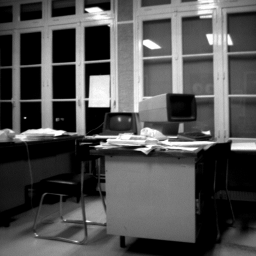
\includegraphics[width=6cm]{Images/office.png}}};
	\node(a)[anchor=center, xshift=3.2cm, yshift=-0.5cm]{\centerline{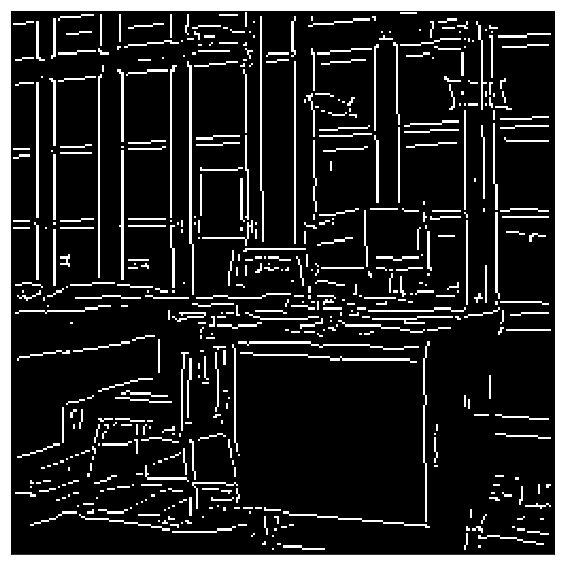
\includegraphics[width=6.2cm]{Images/office_contours.png}}};
    \end{tikzpicture}    	
\end{figure}

\end{frame}

\begin{frame}
\frametitle{ELSB : Edge Least Significant Bit Embedding (4/4)}
\framesubtitle{Explication de l'implémentation \-- \textbf{Insertion du message dans les contours}}

\begin{alertblock}{Choix dans l'implémentation}
\begin{itemize}
    \item[•] on ne modifie que les deux bits de poids faible du rouge
    \item[•] on cache le message dans l'image originale aux coordonnées des contours de l'image masquée 
\end{itemize}
\end{alertblock}

\begin{exampleblock}{Choix dans l'implémentation}
Soit le message : "Il fait beau aujourd'hui" à cacher dans l'image.
\[ \text{1ère lettre du message} = \text{I} ; \text{codeAscii(I)} = 73 ; \text{codeBinaire(} 73 \text{)} = \underbrace{01001001}_{8 bits} \]

\[ \Rightarrow 4 \text{ pixels sont nécessaires pour cacher chaque caractère du message} \]
\end{exampleblock}

\end{frame}

\begin{frame}
\frametitle{Stéganographie dans le domaine fréquentiel}
\framesubtitle{Description théorique}

\begin{block}{Du Spatial au Fréquentiel}
Inconvénients des méthodes relatives au domaine spatial : dégradation de l'image, particulièrement lors d'une compression. \\
\end{block}

\begin{block}{En Pratique}
\begin{itemize}
\item[1] Passage du domaine spatial au domaine fréquentiel : \\
\begin{itemize}
    \item[•] Transformée en Cosinus Discrète (TCD)
    \item[•] Transformée de Fourier Discrète (TFD)
\end{itemize}
\item[2] Le message est intégré aux coefficients transformés
\item[3] Les données sont repassées en spatial (TCD inverse ou TFD inverse)
\end{itemize}

La TCD bidimensionnelle est la transformée la plus utilisée dans le traitement d'images. Une méthode l'exploitant est celle dite "d’incorporation Jpeg-Jsteg", où le message est intégré aux LSB des coefficients TCD dont les valeurs sont différentes de $ 0 $, $ 1 $ et $ -1 $.
\end{block}
\end{frame}

\section{Stéganalyse : détection de la stéganographie}
\begin{frame}
\frametitle{Stéganalyse : détection de la stéganographie}

\begin{block}{Définition}
Vérifier si un document contient une information cachée.
\end{block}

\begin{block}{Plusieurs types de steganalyses}
\begin{itemize}
    \item[•] Passive : Seulement observer le trafic entre l'expéditeur et le destinataire.
    \item[•] Active : Apporter des modifications à l'image
(Compression, filtrage...) avec pour but de détruire le processus stéganographique s’il existe.
    \item[•] "Malicieuse" : Comprendre la technique stéganographique, extraire le message, et l'utiliser à ses propres fins.
\end{itemize}
\end{block}

\begin{block}{Autres types de steganalyses}
\begin{itemize}
    \item[•] Analyser le document pour des méthodes de stéganographie connues (LSB, ELSB, RLSB,...)
    \item[•] Si on possède une version de l'image originale : comparer cette image avec l'image qui contient potentiellement de la stéganographie
\end{itemize}
\end{block}
\end{frame}

\section{Démonstrations}

\section{Conclusion}
\begin{frame}
\frametitle{Conclusion}

\begin{block}{}
On peut cacher différents types d'information dans une image : \\
texte, audio, image, fichier,...
\end{block}

\begin{block}{Différence entre la stéganographie et le tatouage d'image}
\begin{itemize}
    \item[•] Stéganographie : cacher une information dans un document dans le but qu'elle soit indétectable
    \item[•] Tatouage d'image : cacher une information dans un document dans le but qu'elle soit ni retirable, ni modifiable
\end{itemize}
\end{block}

\begin{exampleblock}{La stéganographie aujourd'hui}
Chiffrage de l'information avant de la dissimuler dans une autre
\end{exampleblock}

\begin{alertblock}{Question}
Pourquoi cacher le message sur le bit ou les 2 bits de poids faible de l'image ?
\end{alertblock}

\end{frame}

\section{Bibliographie}
\begin{frame}
\frametitle{Bibliographie (1/3)}
	
\begin{itemize}
\item[•] Analysis and Implementation of Distinct Steganographic Methods
\item[] \url{https://arxiv.org/pdf/1108.2153.pdf}
\item[•] Dissimulation de données : La stéganographie
\item[] \url{https://www.securiteinfo.com/attaques/divers/steganographie.shtml}
\item[•] Ondelette : Tatouage et Stéga-analyse
\item[] \url{https://jnsecurite2018.sciencesconf.org/data/pages/slides_philippe_carre.pdf}
\item[•] La stéganographie au cours des siècles
\item[] \url{http://www.bibmath.net/crypto/index.php?action=affiche&quoi=stegano/histstegano}
\item[•] Some New Methodologies for Image Hiding using Steganographic Techniques
\item[] \url{https://arxiv.org/pdf/1211.0377.pdf}
\end{itemize}
\end{frame}

\begin{frame}
\frametitle{Bibliographie (2/3)}
	
\begin{itemize}
\item[•] A Survey on LSB Based Steganography Methods
\item[] \url{https://www.google.com/url?sa=t&rct=j&q=&esrc=s&source=web&cd=1&ved=2ahUKEwiEsdeQg_reAhWk34UKHShRAj8QFjAAegQICRAC&url=https\%3A\%2F\%2Fwww.ijecs.in\%2Findex.php\%2Fijecs\%2Farticle\%2Fdownload\%2F1912\%2F1767\%2F&usg=AOvVaw3GtnKqK9NY-hwX8vY-i69l}
\item[•] EDGE Based Image Steganography for Data Hiding
\item[]  \url{https://www.google.com/url?sa=t&rct=j&q=&esrc=s&source=web&cd=3&ved=2ahUKEwiB6qrwl_reAhUOYxoKHRF-DmcQFjACegQIBBAC&url=https\%3A\%2F\%2Fpen2print.org\%2Findex.php\%2Fijr\%2Farticle\%2Fdownload\%2F9461\%2F9127&usg=AOvVaw1tXVWLzjun-sY6lRSgbllH}
\item[•] Steganography and Watermarking - FI MUNI
\item[] \url{https://www.google.com/url?sa=t&rct=j&q=&esrc=s&source=web&cd=20&ved=2ahUKEwj179bM_IvfAhUMQRoKHU6MDg4QFjATegQICBAC&url=https\%3A\%2F\%2Fwww.fi.muni.cz\%2Fusr\%2Fgruska\%2Fcrypto09\%2FCRYPTO0911a.ppt&usg=AOvVaw0MnwM9FILA5qt85QxsKPeC}
\end{itemize}
\end{frame}

\begin{frame}
\frametitle{Bibliographie (3/3)}
	
\begin{itemize}
\item[•] A Secure Steganographic Algorithm Based on Frequency Domain for the Transmission of Hidden Information
\item[] \url{https://www.hindawi.com/journals/scn/2017/5397082/}
\item[•]  Le marquage dans le domaine fréquentiel
\item[] \url{http://cours-info.iut-bm.univ-fcomte.fr/wiki/pmwiki.php/Imagerie/Steganographie\#toc10}
\item[•]  Dissimulation de Données
\item[] \url{https://www.google.com/url?sa=t&rct=j&q=&esrc=s&source=web&cd=1&cad=rja&uact=8&ved=2ahUKEwjFnIrs5JLfAhVMRBoKHRnEAH4QFjAAegQIABAC&url=https\%3A\%2F\%2Fwww.lirmm.fr\%2F~wpuech\%2Fenseignement\%2Fmaster_informatique\%2FCompression_Insertion\%2FDissimulation_de_donnees_Cours3.pdf&usg=AOvVaw02tZo9hxXDCYPS8pWcdRfy}
\end{itemize}
\end{frame}
\end{document}